%%%%%%%%% BODY TEXT
\section{Introduction}
\label{sec:intro} 
Visual activity progress prediction is vital to our day-to-day lives: \eg in cooking, we predict how fast the food is ready; in healthcare, estimating how long a surgery will take allows for better resource allocation and shorter waiting times. 
Here, we define activity progress prediction as the task of predicting the percentage of completion of an activity in a video in an online setting, \ie: without access to the length of the video.   
For our purpose, each video contains a single activity, which covers the complete duration of the video and may consist of multiple phases.
However, we assume there are no phase annotations available, as is generally the case in real-world scenarios. 
The main challenge for progress prediction is extracting meaning from the visual inputs, which, ideally relates to the specific phases of the activity and, thus, enables predicting progress.

To address this challenge, current methods rely on deep networks, such as \textsl{VGG-16} \cite{simonyan2015}, \textsl{ResNet} \cite{he2015}, \textsl{YOLOv2} \cite{redmon2016}, or \textsl{I3D} \cite{carreira2018} to extract visual information. 
Furthermore, to remember information over time, current progress prediction methods \cite{becattini2017,twinanda2019} rely on memory blocks and recurrent connections \cite{hochreiter1997long}.
While these embeddings and recurrent connections are useful for extracting visual information and keeping track of the activity progression over time, they may also overfit to uninformative artifacts. 
Here, we aim to analyze if such undesirable learning strategies are occurring when performing progress prediction.

To this end, we consider the state-of-the-art progress prediction methods \cite{becattini2017,kukleva2019,twinanda2019}, as well as two more simple learning-based methods: a 2$D$-only \textsl{ResNet}, and a \textsl{ResNet} model augmented with recurrent connections. 
We evaluate all these learning methods across three video datasets used for progress prediction: \textsl{UCF101-24} \cite{soomro2012}, \textsl{Breakfast} \cite{kuehne2014, kuehne2016}, and \textsl{Cholec80} \cite{twinanda2016}.
Additionally, we compare the learning-based methods with simple non-learning baseline methods such as simply frame counting.

We evaluate models on various dataset types and regimes. We examine the learning methods when they are presented with the full videos during training. In addition, to avoid overfitting to absolute time\slash frame progression, we also evaluate methods when trained on randomly sampled video segments. 
For randomly sampling video segments, it is not possible to do frame-counting, and only the visual information is available for activity progress prediction.
If the methods should fail to extract useful information from the visual data, they would perform on par with non-learning methods based on frame-counting.
Finally, we design a precisely controlled synthetic progress prediction dataset, \textsl{Progress-bar}, on which the visual information is directly related to the progress.
\begin{figure*}[t!]  
    \centering
    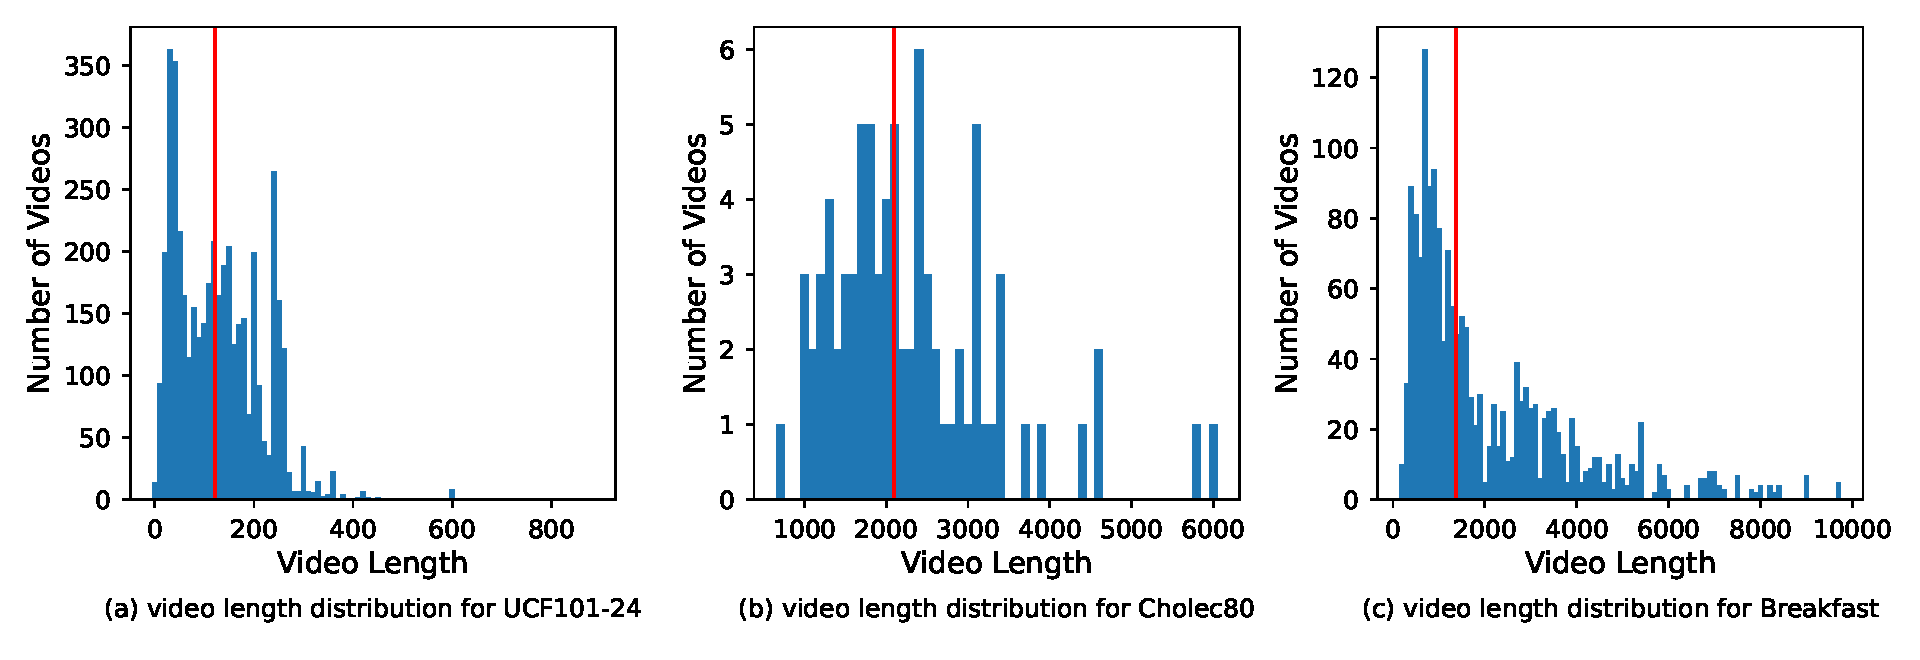
\includegraphics[width=.9\linewidth]{media/dataset_lengths.pdf}
    \caption{
        Length distributions for \textsl{UCF101-24}, \textsl{Cholec80}, and \textsl{Breakfast}. \textsl{UCF101-24} are grouped into bins of size 10, for \textsl{Cholec80} and \textsl{Breakfast} the bins are of size 100. 
        Most notable is the long-tail distribution of the video lengths in the \textsl{Breakfast} dataset, which makes progress prediction difficult. 
        The vertical red line depicts the mean of each dataset.
   }
    \label{fig:lengths}
\end{figure*}

%-------------------------------------------------------
\medskip\noindent\textbf{Difficulties in current progress prediction.}
Progress prediction methods \cite{becattini2017, kukleva2019, twinanda2019} evaluate on complicated and realistic datasets such as \textsl{UCF101-24} \cite{soomro2012}, \textsl{Breakfast} \cite{kuehne2014, kuehne2016}, and \textsl{Cholec80} \cite{twinanda2016}. 
The appearance of the activities in these videos is diverse. 
And the activity length drastically varies between videos in these datasets, as shown \fig{lengths}.
\textsl{UCF101-24} and \textsl{Breakfast} follow a long-tail distribution, with few videos containing long activities.
Moreover, there can be unexpected activity progressions: \eg the pancake gets burned, or there is a surgery lag. 
Also, some of the activities in these datasets do not have a clearly defined endpoint: \eg `skiing', `walking the dog', etc. 
Predicting progress on these activities would be difficult even for a human observer. 
Therefore, we arrive at two main questions we aim to address here: 
(i) \textsl{How well can methods predict activity progression on the current datasets?} and 
(ii) \textsl{Is it at all possible to predict progress from visual data only?}

